\newif\ifglobal

%%%%%%%%%%%%%%%%%%%%%%%
%%% Compile to view %%%
%%%%%%%%%%%%%%%%%%%%%%%

%%%%%%%%%%%%%%%%%%%%%%%%%%%%%%%%%%%%%%%%%%%%%%%%%%%
%%% Readme:                                     %%%
%%% https://www.overleaf.com/read/bwdjvfjksvjy/ %%%
%%%%%%%%%%%%%%%%%%%%%%%%%%%%%%%%%%%%%%%%%%%%%%%%%%%

% >>> M?: marks a module setting number or important notice

% >>> M4: Set {./relative-path} to external files for this module <<<
\def \modulefiles {./02-RESCLK}
% To add an external file, use:
% (Replace '---' with actual filename)
% '\input{\modulefiles/tables/---.tex}' for tables
% '\includegraphics{\modulefiles/figures/---}' for figures
% '\subfile{\modulefiles/---}' for register files


% >>> M1: This module is in global project? <<<
% 'YES' - uncomment; 'NO' - comment out
\globaltrue

\ifglobal
    \documentclass[main\_\_EN.tex]{subfiles}

\else
    \documentclass[openany, 10pt]{book}

    % >>> M2: In ./00-shared/preamble-trm-module, also find
    %         settings for visibility of todo notes, watermark <<<
    \usepackage{preamble-trm-module}

    % >>> M3: Temporary labels in English,
    %         you can add your own labels there <<<
    \myexternaldocument{./00-shared/temp-labels-en}

\fi %\ifglobal


\setcounter{secnumdepth}{4}


% >>> M5: If this module needs any updates in
% './00-shared/preamble-trm-module.sty'
% (include additional package, etc.), contact your module PM
% or create the file './00-shared/changelog.tex' make the
% necessary updates yourself and document them in this file <<<


\begin{document}


% Sets language into which pre-defined bits of text are translated
\selectlanguage{english}

% Do not delete this block
\ifglobal
% Add the following front matter if
% this module is outside of global project
\else
    \InputIfFileExists{readme}{}{}
    {\let\clearpage\relax \listoftodos}
    \tableofcontents
    %\listoftables
    %\listoffigures
\fi


%%%%%%%%%%%%%%%%%%%%%%%%%
%%% TRM Module Begins %%%
%%%%%%%%%%%%%%%%%%%%%%%%%

\hypertarget{resclk}{}
\chapter{Reset and Clock}
\label{mod:resclk}

\section{Reset}
\subsection{Overview}
\chipname{} provides four types of reset that occur at different levels, namely CPU Reset, Core Reset, System Reset, and Chip Reset. All reset types mentioned above (except Chip Reset) maintain the data stored in internal memory. Figure \ref{figure:Reset} shows the scope of affected subsystems by each type of reset.

\subsection{Architectural Overview}
\begin{figure}[H]
    \centering
    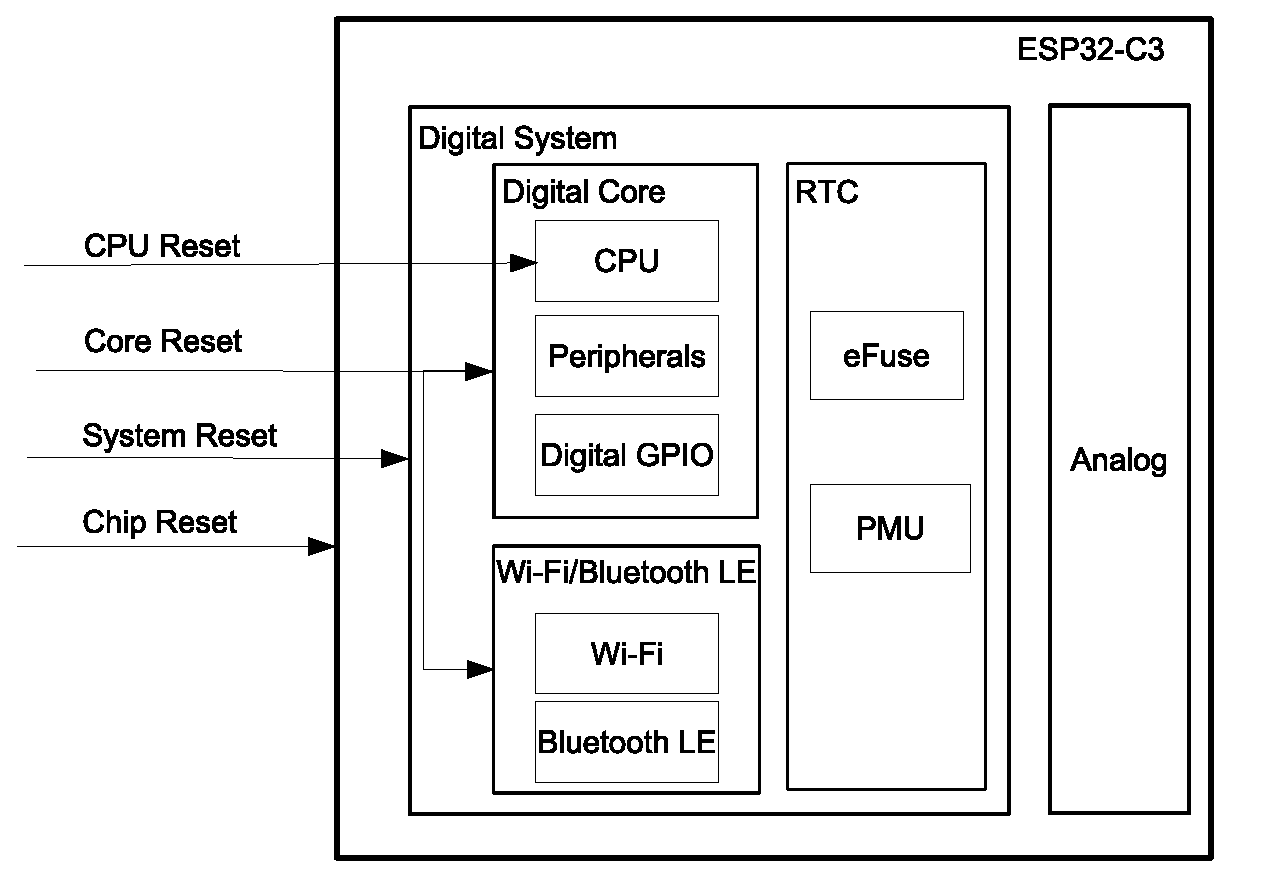
\includegraphics[width=0.8\textwidth]{./02-RESCLK/figures/reset-overview-20210402.eps}
    \caption{Reset Types}
    \label{figure:Reset}
\end{figure}

\subsection{Features}
\begin{itemize}
    \item Support four reset levels:
    \begin{itemize}
    \item CPU Reset: Only resets CPU core. Once such reset is released, the instructions from the CPU reset vector will be executed.
    \item Core Reset: Resets the whole digital system except RTC, including CPU, peripherals, Wi-Fi, Bluetooth$^®$ LE, and digital GPIOs.
    \item System Reset: Resets the whole digital system, including RTC.
    \item Chip Reset: Resets the whole chip.
    \end{itemize}
    \item Support software reset and hardware reset:
    \begin{itemize}
        \item Software Reset: the CPU can trigger a software reset by configuring the corresponding registers, see Chapter \ref{mod:lowpowm} \textit{\nameref{mod:lowpowm}}.
        \item Hardware Reset: Hardware reset is directly triggered by the circuit.
    \end{itemize}
\end{itemize}
\begin{tiplisting}
If CPU is reset, \hyperref[mod:permctrl]{PMS registers} will be reset, too.
\end{tiplisting}

\vspace{-2em}
\subsection{Functional Description}
CPU will be reset immediately when any of the reset above occurs. Users can get reset source codes by reading register RTC\_CNTL\_RESET\_CAUSE\_PROCPU after the reset is released.

Table \ref{tab:resclk-reset-src} lists possible reset sources and the types of reset they trigger.

\begin{table}[H]
    \centering
    \caption{Reset Sources}
    \label{tab:resclk-reset-src}
    \begin{threeparttable}
    \begin{tabular}{ | l | m{3.7cm} | m{2.1cm} | m{8.9cm} | }
    \hline
        \rowcolor{lightgray}
        \textbf{Code} & \textbf{Source} & \textbf{Reset Type} &   \textbf{Comments} \\\hline
        0x01 & Chip reset\tnote{1}  & Chip Reset  & -\\
        \hline
        0x0F & Brown-out system reset  & Chip Reset or System Reset  & Triggered by brown-out detector\tnote{2}\\
        \hline
        0x10 & RWDT system reset  & System Reset  & See Chapter  \ref{mod:wdt} \textit{\nameref{mod:wdt}}
        \\\hline
        0x12 & Super Watchdog reset & System Reset & See Chapter  \ref{mod:wdt} \textit{\nameref{mod:wdt}}
        \\\hline
        0x13 & CLK GLITCH reset  & System Reset  & See Chapter  \ref{mod:glitch} \textit{\nameref{mod:glitch}}
        \\\hline
        0x03 & Software system reset & Core Reset  & Triggered by configuring  RTC\_CNTL\_SW\_SYS\_RST \\
        \hline
        0x05 & Deep-sleep reset  & Core Reset  & See Chapter  \ref{mod:lowpowm} \textit{\nameref{mod:lowpowm}}
        \\\hline
        0x07 & MWDT0 core reset & Core Reset  & See Chapter  \ref{mod:wdt} \textit{\nameref{mod:wdt}}
        \\\hline
        0x08 & MWDT1 core reset & Core Reset  & See Chapter  \ref{mod:wdt} \textit{\nameref{mod:wdt}}
        \\\hline
        0x09 & RWDT core reset  & Core Reset & See Chapter  \ref{mod:wdt} \textit{\nameref{mod:wdt}}
        \\\hline
        0x14 & eFuse reset & Core Reset  & Triggered by eFuse CRC error
        \\\hline
        0x15 & USB (UART) reset & Core Reset & Triggered when external USB host sends a specific command to the Serial interface of USB-Serial-JTAG. See \ref{mod:usbserialjtag} \textit{\nameref{mod:usbserialjtag}} \\\hline
        0x16 & USB (JTAG) reset & Core Reset & Triggered when external USB host sends a specific command to the JTAG interface of USB-Serial-JTAG. See \ref{mod:usbserialjtag} \textit{\nameref{mod:usbserialjtag}}\\\hline

        0x17 & Power glitch reset & Core Reset & Triggered by power glitch
        \\\hline
        0x0B & MWDT0 CPU reset & CPU Reset & See Chapter  \ref{mod:wdt} \textit{\nameref{mod:wdt}}
        \\\hline
         0x0C & Software CPU reset  & CPU Reset  & Triggered by configuring  RTC\_CNTL\_SW\_PROCPU\_RST \\
        \hline
        0x0D & RWDT CPU reset & CPU Reset & See Chapter  \ref{mod:wdt} \textit{\nameref{mod:wdt}}
        \\\hline
        0x11 & MWDT1 CPU reset & CPU Reset & See Chapter  \ref{mod:wdt} \textit{\nameref{mod:wdt}}
        \\\hline
        \end{tabular}

        \begin{tablenotes}
            \item[1]  Chip Reset can be triggered by the following two sources:
    \begin{itemize}
        \item Triggered by chip power-on.
        \item Triggered by brown-out detector.
    \end{itemize}
  \item[2] Once brown-out status is detected, the detector will trigger System Reset or Chip Reset, depending on register configuration. See Chapter  \ref{mod:lowpowm} \textit{\nameref{mod:lowpowm}}.
        \end{tablenotes}
     \end{threeparttable}
    \end{table}

\section{Clock}

\subsection{Overview}

\chipname{} clocks are mainly sourced from oscillator (OSC), RC, and PLL circuit, and then processed by the dividers or selectors, which allows most functional modules to select their working clock according to their power consumption and performance requirements. Figure  \ref{figure:Clock} shows the system clock structure.

\subsection{Architectural Overview}

\begin{figure}[H]
    \centering
    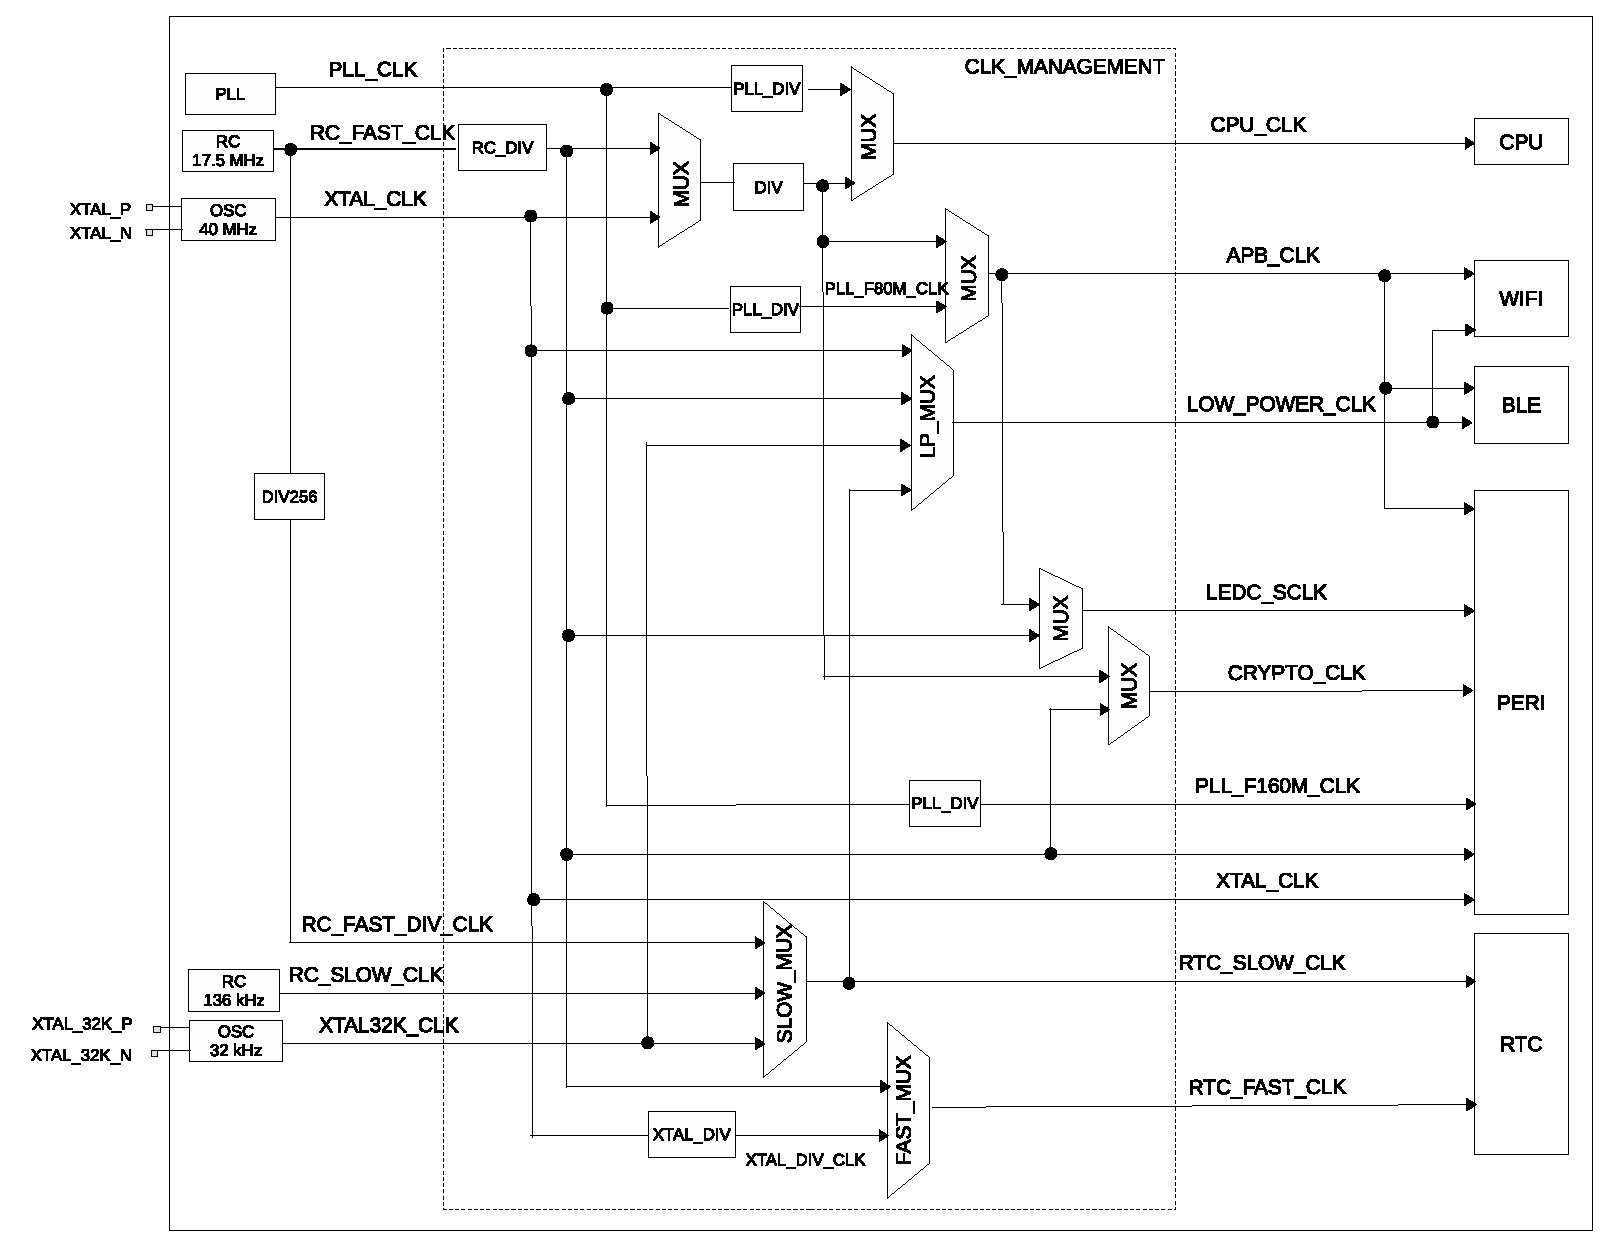
\includegraphics[width=1.0\textwidth]{./02-RESCLK/figures/sys_clk_struct_20250205.eps}
    \caption{System Clock}
    \label{figure:Clock}
\end{figure}

\subsection{Features}

\chipname{} clocks can be classified in two types depending on their frequencies:
\begin{itemize}
    \item High speed clocks for devices working at a higher frequency, such as CPU and digital peripherals
    \begin{itemize}
        \item PLL\_CLK (320 MHz or 480 MHz): internal PLL clock
        \item XTAL\_CLK (40 MHz): external crystal clock
    \end{itemize}
    \item Slow speed clocks for low-power devices, such as RTC module and low-power peripherals
    \begin{itemize}
        \item XTAL32K\_CLK (32 kHz): external crystal clock
	    \item RC\_FAST\_CLK (17.5 MHz by default): internal fast RC oscillator with adjustable frequency
	    \item RC\_FAST\_DIV\_CLK: internal fast RC oscillator derived from RC\_FAST\_CLK divided by 256
	    \item RC\_SLOW\_CLK (136 kHz by default): internal low RC oscillator with adjustable frequency
    \end{itemize}
\end{itemize}

\subsection{Functional Description}

\subsubsection{CPU Clock}

As Figure \ref{figure:Clock} shows, CPU\_CLK is the master clock for CPU and it can be as high as 160 MHz when CPU works in high performance mode. Alternatively, CPU can run at lower frequencies, such as at 2 MHz, to lower power consumption.
Users can set PLL\_CLK, RC\_FAST\_CLK or XTAL\_CLK as CPU\_CLK clock source by configuring register  SYSTEM\_SOC\_CLK\_SEL, see Table  \ref{tab:resclk-cpu-clk-src} and Table  \ref{tab:resclk-cpu-clk-freq}. By default, the CPU clock is sourced from XTAL\_CLK with a divider of 2, i.e. the CPU clock is 20 MHz.

\begin{longtable}[c]{|p{5cm}|p{4cm}| }
       \caption{CPU Clock Source}
		\label{tab:resclk-cpu-clk-src} \\
	    \hline
        \rowcolor{lightgray}
         \textbf{SYSTEM\_SOC\_CLK\_SEL Value} &  \textbf{CPU Clock Source} \\\hline
         \endfirsthead

       \multicolumn{2}{c}{\bfseries \tablename\ \thetable{} -- cont'd from previous page}\\\hline
       \rowcolor{lightgray}
         \textbf{SYSTEM\_SOC\_CLK\_SEL Value} &  \textbf{CPU Clock Source} \\\hline
         \endhead

    \multicolumn{2}{r}{\textbf{Cont'd on next page}} \\
    \endfoot
    \endlastfoot
    \hline
        0 & XTAL\_CLK \\
        \hline
        1 & PLL\_CLK \\
        \hline
        2 & RC\_FAST\_CLK \\
        \hline
\end{longtable}


\begin{table}[H]
    \centering
    \caption{CPU Clock Frequency}
    \label{tab:resclk-cpu-clk-freq}

    \begin{threeparttable}
    \begin{tabular}{ |p{3.0cm}|r|r|r|p{9.0cm}|}
    \hline
        \rowcolor{lightgray}
        \textbf{CPU Clock Source} & \textbf{SEL\_0*} & \textbf{SEL\_1*} & \textbf{SEL\_2*} & \textbf{CPU Clock Frequency} \\
        \hline
		\multirow{2}{*} {XTAL\_CLK} & \multirow{2}{*} {0} & \multirow{2}{*} {-} & \multirow{2}{*} {-} & CPU\_CLK = XTAL\_CLK/(SYSTEM\_PRE\_DIV\_CNT + 1) \newline
         		SYSTEM\_PRE\_DIV\_CNT ranges from 0 \verb+~+ 1023. Default is 1 \\
        \hline
       \multirow{2}{*} {PLL\_CLK (480 MHz)} & \multirow{2}{*} {1} & \multirow{2}{*} {1} & \multirow{2}{*} {0} & CPU\_CLK = PLL\_CLK/6 \newline
         		CPU\_CLK frequency is 80 MHz \\
        \hline
       \multirow{2}{*} {PLL\_CLK (480 MHz)} & \multirow{2}{*} {1} &\multirow{2}{*} {1} & \multirow{2}{*} {1}  & CPU\_CLK = PLL\_CLK/3 \newline
       			CPU\_CLK frequency is 160 MHz \\
        \hline
        \multirow{2}{*} {PLL\_CLK (320 MHz)}  & \multirow{2}{*} {1}  & \multirow{2}{*} {0} & \multirow{2}{*} {0}  & CPU\_CLK = PLL\_CLK/4 \newline
       			CPU\_CLK frequency is 80 MHz \\
        \hline
        \multirow{2}{*} {PLL\_CLK (320 MHz)}  & \multirow{2}{*} {1}  & \multirow{2}{*} {0} & \multirow{2}{*} {1}  & CPU\_CLK = PLL\_CLK/2 \newline
       			CPU\_CLK frequency is 160 MHz \\
        \hline
       \multirow{2}{*} {RC\_FAST\_CLK}  & \multirow{2}{*} {2}  & \multirow{2}{*} {-}  & \multirow{2}{*} {-} & CPU\_CLK = RC\_FAST\_CLK/(SYSTEM\_PRE\_DIV\_CNT + 1) \newline
        		SYSTEM\_PRE\_DIV\_CNT ranges from 0 \verb+~+ 1023. Default is 1 \\
        \hline
    \end{tabular}

        \begin{tablenotes}
            \item[*] The value of SYSTEM\_SOC\_CLK\_SEL.
            \item[*] The value of SYSTEM\_PLL\_FREQ\_SEL.
            \item[*] The value of SYSTEM\_CPUPERIOD\_SEL.
        \end{tablenotes}
     \end{threeparttable}
    \end{table}

\subsubsection{Peripheral Clock}
Peripheral clocks include APB\_CLK, CRYPTO\_CLK, PLL\_F160M\_CLK, LEDC\_SCLK, XTAL\_CLK, and RC\_FAST\_CLK. Table \ref{tab:resclk-periph-clks} shows which clock can be used by each peripheral.

\begin{landscape}
\begin{longtable}[c]{|p{2.5cm}|c|c|c|c|c|c|c|c| }
 \caption{Peripheral Clocks}
    \label{tab:resclk-periph-clks} \\
  \hline
        \rowcolor{lightgray}
        \textbf{Peripheral} &  \textbf{XTAL\_CLK} &  \textbf{APB\_CLK} &  \textbf{PLL\_F160M\_CLK} &  \textbf{RTC\_FAST\_CLK} &  \textbf{RC\_FAST\_CLK} &  \textbf{CRYPTO\_CLK} &   \textbf{LEDC\_CLK} &  \textbf{PLL\_D2\_CLK}  \\\hline
        \endfirsthead

       \multicolumn{9}{c}{\bfseries \tablename\ \thetable{} -- cont'd from previous page}\\\hline
       \rowcolor{lightgray}
        \textbf{Peripheral} &  \textbf{XTAL\_CLK} &  \textbf{APB\_CLK} &  \textbf{PLL\_F160M\_CLK} & \textbf{RC\_FAST\_CLK} &  \textbf{CRYPTO\_PWM\_CLK} &   \textbf{LEDC\_CLK} & \textbf{PLL\_D2\_CLK}  \\\hline
        \endhead

    \multicolumn{9}{r}{\textbf{Cont'd on next page}} \\
    \endfoot
    \endlastfoot
    \hline
        TIMG & Y & Y &   &   &   & & &\\
        \hline
        I2S  & Y &   & Y &  &   & & & Y\\
        \hline
        UHCI &  & Y   &   &   &   & & &\\
        \hline
        UART & Y & Y   &   &   & Y & & &\\
        \hline
        RMT  & Y & Y   &   &   & Y & & &\\
        \hline
        I2C  & Y &   &   &   & Y & & &\\
        \hline
        SPI  & Y & Y   &   &   &   & & &\\
        \hline
        eFuse Controller &  Y &   & & Y & & & &\\
        \hline
        SARADC &   & Y    &   &   &   & & &\\
        \hline
        Temperature Sensor &  Y &     &   &   &  Y & & & \\
        \hline
        USB &   & Y    &   &   &   & & & \\
        \hline
        CRYPTO  &   &      &   &   &   &Y & &\\
        \hline
        TWAI Controller &  & Y   &  & & & & &\\
        \hline
        LEDC & Y&  Y   &Y &   &  Y & & Y &\\
        \hline
        SYS\_TIMER& Y & Y   &   &   &   & & &\\
        \hline
\end{longtable}
\end{landscape}

\textbf{APB\_CLK}

The frequency of APB\_CLK is determined by the clock source of CPU\_CLK as shown in Table  \ref{tab:resclk-apb-clk-freq}.

\begin{longtable}[c]{ |p{5cm}|p{5cm}| }
\caption{APB\_CLK Clock Frequency}\label{tab:resclk-apb-clk-freq}
\\\hline
    \rowcolor{lightgray}
        \textbf{CPU\_CLK Source} & \textbf{APB\_CLK Frequency} \\
        \hline
        \endfirsthead

        \multicolumn{2}{c}{\bfseries \tablename\ \thetable{} -- cont'd from previous page}\\\hline

        \rowcolor{lightgray}
        \textbf{CPU\_CLK Source} & \textbf{APB\_CLK Frequency}\\
        \hline
        \endhead
        \multicolumn{2}{r}{\textbf{Cont'd on next page}} \\
        \endfoot
        \endlastfoot
        \hline
        PLL\_CLK & 80 MHz \\
        \hline
        XTAL\_CLK & CPU\_CLK \\
        \hline
        RC\_FAST\_CLK & CPU\_CLK \\
        \hline
\end{longtable}


\textbf{CRYPTO\_CLK }

The frequency of CRYPTO\_CLK is determined by the CPU\_CLK source, as shown in Table  \ref{tab:resclk-crypto-clk-freq}.

 \begin{longtable}[c]{ |p{5cm}|p{5.5cm}| }
      \caption{CRYPTO\_CLK Frequency}
    \label{tab:resclk-crypto-clk-freq} \\
        \hline
        \rowcolor{lightgray}
        \textbf{CPU\_CLK Source} & \textbf{CRYPTO\_CLK Frequency} \\
        \hline
        \endfirsthead
        \multicolumn{2}{c}{\bfseries \tablename\ \thetable{} -- cont'd from previous page}\\\hline
        \rowcolor{lightgray}
        CPU\_CLK Source & CRYPTO\_CLK Frequency \\
        \hline
        \endhead
        \multicolumn{2}{r}{\textbf{Cont'd on next page}} \\
        \endfoot
        \endlastfoot
        \hline
        PLL\_CLK & 160 MHz \\
        \hline
        XTAL\_CLK & CPU\_CLK \\
        \hline
        RC\_FAST\_CLK & CPU\_CLK \\
        \hline
\end{longtable}

\textbf{PLL\_F160M\_CLK }

PLL\_F160M\_CLK is divided from PLL\_CLK according to current PLL frequency.


\textbf{LEDC\_SCLK}

LEDC module uses RC\_FAST\_CLK as clock source when APB\_CLK is disabled. In other words, when the system is in low-power mode, most peripherals will be halted (as APB\_CLK is turned off), but LEDC can still work normally via RC\_FAST\_CLK.

\subsubsection{Wi-Fi and Bluetooth LE Clock}
Wi-Fi and Bluetooth LE can only work when CPU\_CLK uses PLL\_CLK as its clock source. Suspending PLL\_CLK requires that Wi-Fi and  Bluetooth LE have entered low-power mode first.

LOW\_POWER\_CLK uses XTAL32K\_CLK, XTAL\_CLK, RC\_FAST\_CLK or RTC\_SLOW\_CLK (the low clock selected by RTC) as its clock source for Wi-Fi and Bluetooth LE in low-power mode.


\subsubsection{RTC Clock}

The clock sources for RTC\_SLOW\_CLK and RTC\_FAST\_CLK are low-frequency clocks. RTC module can operate when most other clocks are stopped. RTC\_SLOW\_CLK derived from RC\_SLOW\_CLK, XTAL32K\_CLK or RC\_FAST\_DIV\_CLK is used to clock Power Management module. RTC\_FAST\_CLK is used to clock On-chip Sensor module. It can be sourced from a divided XTAL\_CLK or from a divided RC\_FAST\_CLK.


\end{document}
